\chapter{Réalisations}\label{chap:realisations}

	Dans ce chapitre, je détaille la seconde partie de mon travail de recherche :
	mes réalisations. En effet, ma mission était d'aider à finir l'article en
	cours d'écriture, dont j'ai présenté l'existant dans la section
	\ref{sec:mls_dynamic}. Ce chapitre présentera donc les travaux que j'ai
	réalisés pour aider à la finition de cet article.

	La première de mes réalisations a été de calculer la probabilité de créer un
	bloc pour un adversaire, sachant que celui-ci peut tricher sur la target $T$
	qu'il choisit. On a ensuite cherché à déterminer une valeur de $m$ qui
	permettrait de garantir les propriétés souhaitées pour l'algorithme MLS. Pour
	cela, on a exploré deux méthodes : une méthode par marche aléatoire, et une
	méthode par la ruine du joueur. La méthode par marche aléatoire n'a rien
	donné, le problème n'étant pas résolu à l'heure actuelle par la communauté
	scientifique. En revanche, la méthode par la ruine du joueur a fourni des
	outils pour déterminer la valeur de $m$ en fonction de la quantité de triche
	de l'adversaire. Enfin, dans la dernière section de ce chapitre, je parlerai
	des activités que j'ai réalisées durant mon stage, en marge de ce sujet.


\section{Probabilité de créer un bloc}\label{sec:probabilite-bloc}

	Mon premier travail a été de calculer la probabilité qu'un bloc appartienne à
	un adversaire. En effet, on aura besoin de cette probabilité pour calculer la
	valeur de $m$ par la suite.

	Dans une même ronde, on a quatre situations possibles : aucun bloc n'est créé,
	seul l'honnête crée un bloc, seul l'adversaire crée un bloc, ou les deux
	créent un bloc. On cherche la probabilité $\mu$ qu'un seul bloc soit créé, et
	que ce bloc appartienne à l'adversaire. On considère uniquement le cas où seul
	l'adversaire crée un bloc, car c'est le cas le plus intéressant pour
	l'adversaire. En effet, si les deux parties créent un bloc en même temps, on
	est dans une situation de fork et ce sont les blocs futurs qui vont décider de
	laquelle des deux versions de la chaîne sera acceptée. Il est donc plus
	intéressant pour l'adversaire de créer un bloc seul, pour être sûr que son
	bloc soit accepté.

	Il est légitime que deux nœuds aient des targets différentes jusqu'à un
	facteur $\alpha$ tel que $\alpha T_m = T_b$. Ainsi, si $\alpha = 1/4$, la
	target de l'adversaire est 4 fois plus faible que celle de l'honnête, il est
	donc 4 fois plus difficile pour l'adversaire de créer un bloc. Inversement, si
	$\alpha = 4$, la target de l'adversaire est 4 fois plus grande que celle de
	l'honnête, il est donc 4 fois plus facile pour l'adversaire de créer un bloc.

	On nomme $N$ la variable aléatoire qui représente le nombre de blocs créés
	durant une ronde. On appelle $B$ l'événement "un bloc de la ronde appartient à
	Bob" (Bob est l'honnête), $M$ l'événement "un bloc de la ronde appartient à
	Mallory" (Mallory est l'adversaire). Calculer la probabilité $\mu(\alpha)$
	qu'un bloc appartienne à Mallory revient à se demander : sachant qu'un seul
	bloc a été crée durant la ronde, quelle est la probabilité que ce bloc
	appartienne à Mallory ? Plus formellement, on cherche à calculer $\mu(\alpha)
	= P(M | N=1)$. De manière assez intuitive, on peut dire que la probabilité que
	ce bloc appartienne à Bob vaut $1 - \mu(\alpha) = P(B | N=1)$.


	On note  $P_b$ la probabilité pour un unique honnête de créer un bloc en une
	seule requête à la fonction de hash, $P_m$ la probabilité pour un unique
	adversaire de créer un bloc en une seule requête à la fonction de hash, $r$ le
	nombre de requêtes à la fonction de hash par ronde, $n$ le nombre de nœuds
	au total, et $t$ le nombre de nœuds adversariaux. On a donc, à partir de
	l'équation \ref{eq:proba-bloc} du modèle :
	
	\begin{equation}
		P(B) = 1 - (1 - P_b)^{r(n-t)}
	\end{equation}
	\begin{equation}
		P(M) = 1 - (1 - P_m)^{rt}
	\end{equation}
	\begin{equation}
		P(N=1) = P(B \land \neg M) + P(\neg B \land M)
	\end{equation}

	Avec la formule des probabilités conditionnelles :

	\begin{equation}
		P(M | N=1)
		= \frac{P(M \land \neg B)}{P(N=1)}
			  = \frac{
					(1 - (1 - \frac{T_m}{2^\kappa})^{rt})(1 - \frac{T_b}{2^\kappa})^{r(n-t)}
				}
				{
					(1 - \frac{T_b}{2^\kappa})^{r(n-t)} 
					+ (1 - \frac{T_m}{2^\kappa})^{rt} 
					- 2(1 - \frac{T_b}{2^\kappa})^{r(n-t)}(1 - \frac{T_m}{2^\kappa})^{rt}
				}
	\label{eq:m_sachant_n}
	\end{equation}

	Avec $T_b$ la target choisie par l'honnête, et $T_m$ la target choisie par
	l'adversaire.

	\paragraph{Simplification du calcul de $\mu(\alpha)$} Plus tard durant mon
	stage, je me suis rendu compte que l'on pouvait approcher $\mu(\alpha)$ de
	manière plus simple. En effet, si on ne prend pas en compte les collisions
	(c'est à dire les moments ou les deux joueurs trouvent un bloc à la même
	ronde), il suffit de considérer que si l'adversaire mine un bloc 4 fois plus
	difficile ($\alpha = 4$), il le fera 4 fois moins souvent. On a donc
	$\mu(\alpha) = \alpha t/((n-t)+\alpha t)$. Dans les fait, les modèles
	statique~\cite{static_backbone} et dynamique~\cite{dynamic_backbone} nous
	apprennent que les collisions sont extrêmement rare, on peut donc utiliser
	cette approximation sans problème dans la plupart des cas. Malgré tout, dans
	le reste de ce mémoire, toutes les applications numériques ont été faites avec
	la formule complète de $\mu(\alpha)$, la formule \ref{eq:m_sachant_n}.

	Le protocole borne la dérive entre les targets des participants d'un facteur
	$\alpha \in [1/4, 4]$, ce qui implique l'adversaire ne peut pas tricher sur sa
	target plus que d'un facteur 4. En effet, si l'adversaire triche trop, il sera
	immédiatement repéré par les autres nœuds, et le bloc ne sera pas accepté. On
	a donc $T_m/4 \geq T_b \geq 4T_m$.

	On a donc effectué l'application numérique pour les trois valeurs de $\alpha$
	: $\alpha = 1/4$, $\alpha = 1$, et $\alpha = 4$, avec un adversaire à $1/3$ de
	la puissance de calcul ($n = t/3$), puisqu'il s'agit du cas le plus critique
	pour le réseau, tel que décrit dans l'article~\cite{dynamic_backbone}.
	
	Les résultats obtenus sont décrits dans le tableau~\ref{tab:pbbloc}.

	\begin{table}[h]
		\centering
		\begin{tabular}{|c||c|c|}
			\hline
			$\alpha$ & $\mu(\alpha)$ & $1 - \mu(\alpha)$ \\
			\hline
			$1/4$ & $1/9$ & $8/9$ \\
			$1$ & $1/3$ & $2/3$ \\
			$4$ & $2/3$ & $1/3$\\
			\hline
		\end{tabular}
		\caption{$\mu(\alpha)$ en fonction de $\alpha$ avec $q = 1/3$}
		\label{tab:pbbloc}
	\end{table}

	De manière assez intuitive, on peut voir que plus l'adversaire a une target
	grande (donc facile), plus il a de chance de créer un bloc. Quand il triche au
	maximum ($\alpha = 4$), $2/3$ des blocs créés seront des blocs adversariaux,
	contre seulement $1/3$ de blocs honnêtes. Cependant, comme les protocoles
	Bitcoin et MLS ne comparent pas le nombre de blocs entre deux chaînes, mais la
	somme de travail fourni, l'adversaire aura peut-être plus de blocs, mais ils
	auront moins de "valeur" que les blocs honnêtes. Il est donc important de se
	demander quelle serait la meilleure stratégie pour l'adversaire : plus de
	blocs de moins grande valeur, ou moins de blocs de plus grande valeur ? C'est
	une question qu'il faudra prendre en compte dans les calcul de la valeur de
	$m$, et fixer sa valeur de manière à ce que l'algorithme résiste à l'attaque
	de l'adversaire, même dans le pire des cas.


\section{Recherche de \textit{m} par marche
aléatoire}\label{sec:recherche-m-alea}

	Dans l'algorithme MLS, la valeur de $m$ est un paramètre important. C'est le
	paramètre qui va définir le nombre de blocs de chaque niveau de la chaîne. Il
	doit être suffisamment grand pour être sur que l'adversaire ne puisse pas
	rattraper la chaîne honnête, mais pas trop grand pour ne pas créer un
	compressé trop grand. De plus, étant donné que l'adversaire peut tricher sur
	la target, on va trouver plusieurs valeurs de $m$ fonction de la quantité de
	triche $\alpha$ de l'adversaire, on prendra donc le $m$ maximal parmi ces
	valeurs.

	On a donc cherché à déterminer les valeurs de $m$ qui permettraient de
	garantir les propriétés souhaitées pour l'algorithme MLS. Pour commencer, on a
	essayé de modéliser la création de blocs par une marche aléatoire non isotrope
	en deux dimensions.


	\subsection{Construction du modèle}\label{subsec:walk-construction-modele}

	En prenant appui sur l'article~\cite{nca}, qui travaillait sur un problème
	similaire, on a travaillé sur la création d'un modèle permettant de simuler
	la création des blocs. 

	On considère une succession de rondes où l'honnête et l'adversaire jouent
	chacun de leur côté. On s'intéresse au nombre de victoires de chaque joueur
	(Bob et Mallory) après $k$ victoires au total. On note $V_k = (A_b, A_m)$
	l'état après $k$ victoires, où $A_b$ et $A_m$ sont respectivement le nombre de
	victoires de Bob et de Mallory. A partir de l'état $V_k = (A_b, A_m)$, seules
	deux transitions sont possibles : soit Bob gagne la ronde et on a $V_{k+1} =
	(A_b+1, A_m)$, soit Mallory gagne la ronde et on a $V_{k+1} = (A_b, A_m+1)$.
	On note $\mu(\alpha)$ la probabilité que Mallory gagne la ronde, et
	$1-\mu(\alpha)$ la probabilité que Bob gagne la ronde. On ne s'intéresse pas
	aux rondes où aucun bloc n'est créé, car elles n'ont pas d'impact sur la
	chaîne.
	
	L'espace de $V_k$ est donc un quart de plan : si Bob gagne la ronde, on va
	vers la droite, si Mallory gagne la ronde, on va vers le haut. On va tracer
	une droite délimitant l'espace de $V_k$ en deux parties : l'espace
	$\mathcal{B}$ où la chaîne de Bob a plus de difficulté cumulée que la chaîne
	de Mallory, et l'espace $\mathcal{M}$ où la chaîne de Mallory a plus de
	difficultés que la chaîne de Bob. Cet espace est délimité par la droite $A_b -
	\alpha A_m = 0$, de telle manière que :

	\begin{equation}
			\mathcal{M} = \{ (b,m) \in \mathbb{N}^2 \mid A_b - \alpha A_m >= 0 \}
	\end{equation}
	\begin{equation}
			\mathcal{B} = \{ (b,m) \in \mathbb{N}^2 \mid A_b - \alpha A_m < 0 \}
	\end{equation}


	Dans cette définition $V_k \in \mathcal{B}$ signifie que la chaîne de Bob a
	plus de difficulté que la chaîne de Mallory, et $V_k \in \mathcal{M}$
	signifie que la chaîne de Mallory a plus de difficulté que la chaîne de Bob.

	\vspace{0.4cm}
	\begin{figure}[h]
			\centering
			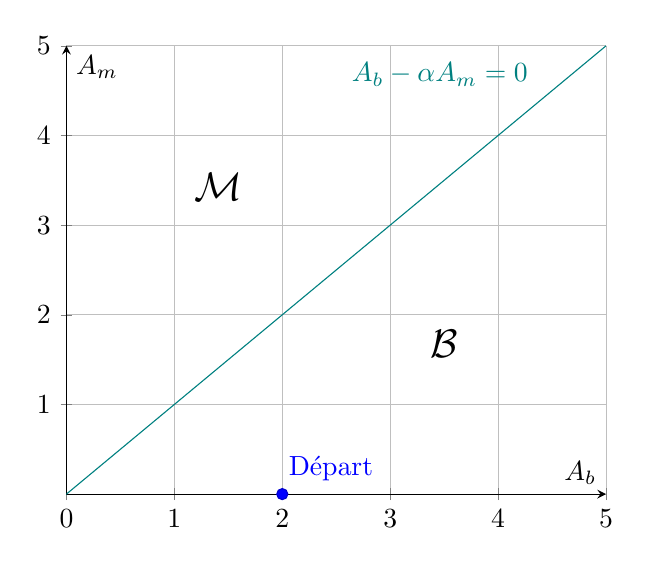
\begin{tikzpicture}
	\begin{axis}[
		grid=major,
		axis lines=middle,
		axis x line=bottom,  
		xlabel=$A_b$,
		ylabel=$A_m$,
		xmin=0,xmax=5,
		ymin=0,ymax=5,
		% xtick={0,...,9},
	]

	\addplot[teal] {\x} node[midway,above]{ };

	\addplot[scatter, only marks, mark=*, mark size=2pt, teal] coordinates {
		(2,0)
	};
	\end{axis}


	\node[anchor=north west, teal] at (3.5, 5.6) {$A_b - \alpha A_m = 0$};
	\node[anchor=north west, blue] at (2.7,0.6) {Départ};
	\node[anchor=north west] at (1.5,4.2) {\Large $\mathcal{M}$};
	\node[anchor=north west] at (4.5,2.2) {\Large $\mathcal{B}$};
\end{tikzpicture}
			\caption{Modélisation de la marche aléatoire pour $m = 2$ et $\alpha = 1$}
			\label{fig:walk}
	\end{figure}

	On part du principe que Bob part avec une avance de $m$ blocs, donc $V_0 = (m,
	0)$. On cherche à déterminer la probabilité que Mallory rattrape Bob, c'est à
	dire la probabilité $P_{\text{gagne}}(m)$ que la marche aléatoire atteigne la
	droite $A_b - \alpha A_m = 0$, sachant que la marche aléatoire a commencé à la
	position $(m, 0)$. $P_{\text{gagne}}(m)$ est décroissante en fonction de $m$ :
	plus Bob part avec une avance grande, moins Mallory a de chances de le
	rattraper. On cherche donc :
	
	\begin{equation}\label{eq:min-m}
		\min_{m \in \mathbb{N}} P_{\text{gagne}}(M) < \varepsilon
	\end{equation}

	Avec $\varepsilon$ notre paramètre de sécurité, la probabilité que Mallory
	rattrape Bob malgré une avance de $m$ blocs. 


	\subsection{Résultats}\label{subsec:walk-resultats}

	Pour calculer la probabilité $P_{\text{gagne}}(m)$, il fallait une fonction
	$f(x,y,x',y', \alpha)$ qui renvoie le nombre de chemins pour aller du point
	$(x,y)$ au point $(x',y')$ sans passer au dessus de la droite $A_b - \alpha
	A_m = 0$. On a assez vite trouvé une formule pouvant nous
	aider~\cite{combinatoire} :

	\begin{equation}\label{eq:f-simple}
		f(x,y,x',y', \alpha) = 
			\binom{(x'-x)+(y'-y)}{x'-x} -
			(\alpha + 1)\binom{(x'-x)+(y'-y)}{y'-y} 
		\forall \alpha \geq 1
	\end{equation}

	Malheureusement, cette expression n'est valable que pour $\alpha \geq 1$. On
	s'est assez vite rendu compte que, malgré l'apparente similarité entre les
	deux cas $\alpha \geq 1$ et $\alpha < 1$, les deux problèmes impliquaient des
	méthodes de résolution différentes. On a donc passé un certain temps à essayer
	de trouver une formule pour $\alpha < 1$. J'ai développé un programme
	permettant de tester nos formules et comparer nos résultats avec ceux obtenus
	par simulation. On a fini par trouver une formule récursive pour $\alpha < 1$
	:

	\begin{equation} 
		f(0,1,x,y) = 
		\binom{x+y-1}{y} - g(y-1) - \sum_{i=0}^{y-2}
		{g(i)\binom{x+y-i-\lfloor{\frac{i+1}{4}\rfloor}-3}
		{y-i-1}}
	\end{equation}
	\vspace{0.3cm}
	\begin{equation}
		g(z) = 
		\sum_{i=1}^{\lceil\frac{z+1}{4}\rceil}
		\left[
			\binom{z+\lceil\frac{z+1}{4}\rceil-i}{z}
			\sum_{j=0}^{z-2}g(j)
			\binom{z+\lfloor\frac{z}{4}\rfloor - j - \lfloor\frac{j+1}
			{4}\rfloor-i-1}{z-j-1}
		\right]
	\end{equation}

	Cette formule permettait de compter le nombre de chemins permettant de relier
	deux points tout en restant strictement en dessous de la droite $A_b - 1/4 A_m
	= 0$., mais uniquement pour un point de départ $(0,1)$. On a donc cherché à
	généraliser cette formule pour un point de départ quelconque $(x,y)$. On a
	finalement trouvé une technique générale permettant de calculer le nombre de
	chemins pour relier deux points $(x,y)$ et $(x',y')$ pour n'importe quel
	$\alpha \leq 1$ dans un ouvrage de combinatoire \cite{combinatoire}.

	Malheureusement, malgré nos efforts, une telle technique n'a pas abouti car
	elle impliquait des outils mathématiques complexes qu'aucun d'entre nous ne
	maîtrisait. On a donc essayé de trouver une autre méthode pour déterminer la
	valeur de $m$, que je décrirai dans la section suivante
	\ref{sec:recherche-m-gamblers-ruin}.

	Malgré tout, nous avions une formule pour $\alpha \geq 1$, et j'ai pu calculer
	une valeur de $m$ pour $\alpha = 1$ et $\alpha = 4$ comme suit :

	\begin{equation}
		P_{\text{gagne}}(m) = 
			\sum_{A_b=m}^{\infty} 
				f(m,0,A_b,\alpha A_m,) 
				\mu(\alpha)^{\alpha A_m}
				(1-\mu(\alpha))^{A_b}
	\end{equation}
	
	Avec $f$ de l'équation \ref{eq:f-simple} pour $\alpha \geq 1$. J'ai pu 
	effectuer l'application numérique pour au moins deux valeurs de $\alpha$ :
	$\alpha = 1$ et $\alpha = 4$. Le tableau~\ref{tab:m_alpha} donne les valeurs
	de $m$ pour un $\varepsilon = 10^{-6}$ et un adversaire détenant $1/3$ de la
	puissance de calcul.
	
	\begin{table}[h]
		\centering
		\begin{tabular}{|c||c|}
			\hline
			$\alpha$ & $m$ \\
			\hline
			$1$ & $65$ \\
			$4$ & $26$ \\
			\hline
		\end{tabular}
		\caption{$m$ en fonction de $\alpha$, avec $q = 1/3$ et $\varepsilon =
		10^{-6}$}
		\label{tab:m_alpha}
	\end{table}

	On peut voir que la valeur de $m$ est plus grande pour $\alpha = 1$ que pour
	$\alpha = 4$. On peut en déduire qu'il sera plus facile pour l'adversaire de
	rattraper l'honnête si l'adversaire mine des blocs à la target officielle, il
	faut donc augmenter la valeur de $m$ pour empêcher l'honnête de se faire
	rattraper. Ces valeurs de $m$ serviront donc pour valider les propriétés du
	second modèle, si on trouve des $m$ dans le même ordre de grandeur, on pourra
	raisonnablement penser que les résultats sont corrects.
	

\section{Recherche de \textit{m} par la ruine du joueur}
\label{sec:recherche-m-gamblers-ruin}

	La recherche de $m$ par la méthode de la marche aléatoire décrite dans la
	section~\ref{sec:recherche-m-alea} n'ayant pas abouti, on a cherché une autre
	méthode pour déterminer les valeurs de $m$ qui permettrait de garantir les
	propriétés souhaitées pour l'algorithme MLS. On est donc parti de l'idée
	originale de Nakamoto, qui a déterminé la probabilité pour l'adversaire de
	rattraper l'honnête en utilisant une loi de Poisson~\cite{bitcoin}. On a donc
	cherché à adapter cette méthode pour notre problème, à savoir déterminer la
	probabilité pour l'adversaire de rattraper l'honnête, sachant que la valeur
	relative entre les blocs honnête et les blocs adversariaux peut varier d'un
	facteur $\alpha$.

	On a utilisé les travaux présenté dans les articles~\cite{rosenfeld}
	et~\cite{double-spend} qui apportent des compléments et des corrections au
	calcul original de Nakamoto. On a ensuite utilisé l'article~\cite{gamblers}
	pour calculer la probabilité de ruine du joueur avec des gains différents des
	pertes, contrairement à la ruine du joueur "classique".


	\subsection{Construction du modèle}\label{subsec:ruin-construction-modele}

	Le modèle de recherche de $m$ par ruine du joueur modélise la progression de
	la chaîne honnête et de la chaîne adversariale par une chaîne de Markov. Dans
	le contexte de la ruine du joueur, on peut dire que l'honnête joue avec un
	solde initial de $m$. À chaque jeu, l'honnête peut gagner avec une probabilité
	$1-\mu(\alpha)$ et perdre avec une probabilité $\mu(\alpha)$. Mais la
	différence avec la ruine du joueur classique, c'est que l'honnête ne perd pas
	la même quantité que ce qu'il gagne. En effet, si l'adversaire mine à une
	target $\alpha = 4$ (donc 4 fois plus facile que l'honnête), l'honnête gagnera
	4 à chaque partie gagnée (\emph{i.e.} un bloc miné), mais l'adversaire gagnera 1 à
	chaque partie gagnée.

	
	\paragraph{Calcul de la probabilité de perte} On s'intéresse donc à la
	probabilité que l'adversaire rattrape l'honnête. En terme de ruine du joueur,
	cela revient à calculer la probabilité que l'honnête soit ruiné. Avec des
	gains différents des pertes, ce calcul est assez complexe. Posons $a$ le gain
	de l'honnête, et $b$ le gain de l'adversaire. Ainsi, si $\alpha = 4$, on a $a
	= 4$ et $b = 1$, si $\alpha = 1$, on a $a = 1$ et $b = 1$ et si $\alpha =
	1/4$, on a $a = 1$ et $b = 4$. Avec les travaux présentés dans les
	articles~\cite{rosenfeld} et~\cite{double-spend}, on a pu déterminer la
	probabilité que l'adversaire rattrape l'honnête malgré une avance de $m$ blocs
	(ou de $m\cdot a$ difficulté) comme suit :

	\begin{equation}\label{eq:prob-gagne}
		P_{\text{gagne}}(m) = 1 - \sum_{k=0}^{ma-1} {
			\frac{\lambda^k e^{-\lambda}}{k!}
			(1 - P_{\text{ruin}}(ma-kb))
		}
	\end{equation}
	\vspace{0.3cm}
	\begin{equation}
		\lambda = \frac{m \mu(\alpha)}{1-\mu(\alpha)}
	\end{equation}

	Il s'agit d'une loi de Poisson de paramètre $\lambda$ représentant le taux de
	création de blocs de l'adversaire et $P_{\text{ruin}}(m)$ la probabilité que
	l'honnête soit ruiné avec un solde de difficulté $ma-kb$.

	\paragraph{Calcul de la probabilité de ruine} C'est donc la valeur de
	$P_{\text{ruin}}(M)$ qui nous reste à déterminer. Il s'agit du calcul de la
	probabilité de ruine du joueur avec des gains différents des pertes. Ce genre
	de calcul est assez complexe, mais l'article~\cite{gamblers} nous à donné des
	pistes pour calculer la probabilité de ruine du joueur dans ce genre de
	situation. On pose une série de Laurent $p(z)$ représentant l'espérance de
	gain du joueur :
	
	\begin{equation}\label{eq:serie-laurent}
		p(z) = (1-\mu(\alpha)) z^{a} + \mu(\alpha) z^{-b} + 1
	\end{equation}

	On cherche ensuite les $\nu$ racines $\eta$ de $p(z)$ dans le disque unité
	$|z| < 1$. La probabilité de ruine du joueur est alors donnée par :

	\begin{equation}\label{eq:ruin-proba}
		P_\text{ruin}(M) = \sum_{j=1}^{\nu} {
			\eta^M_j \prod_{i\neq j} \frac{1 - \eta_i}{\eta_j - \eta_i}
		}	
	\end{equation}

	L'équation~\ref{eq:prob-gagne} nous donne donc la probabilité que l'adversaire
	rattrape l'honnête, sachant que l'honnête à une avance de $M$ difficulté.
	Notre but sera de rendre cette probabilité inférieure à un certain
	$\varepsilon$ pour garantir que l'honnête ne sera pas rattrapé par
	l'adversaire même si celui-ci triche sur la target.

	\paragraph{Vérification du modèle} À l'heure où j'écris ce mémoire, nous 
	sommes en train de refaire les preuves des équations~\ref{eq:serie-laurent}
	et~\ref{eq:ruin-proba} pour être sûr de leur validité. En effet, bien que
	l'article~\cite{gamblers} ai été publié et donc validé par des pairs, il est
	toujours bon de vérifier les résultats. C'est également l'occasion de 
	comprendre en profondeur le fonctionnement de ces équations, et d'être 
	convaincu que l'application que l'on en fait est cohérente avec ce que 
	l'on cherche à modéliser.


	\subsection{Résultats}\label{subsec:ruin-resultats}
	
	Pour trouver les valeurs de $m$ qui permettraient de garantir les propriétés
	souhaitées pour l'algorithme MLS, j'ai développé un programme permettant de
	calculer par recherche dichotomique les valeurs de $m$ pour différentes
	valeurs de $\alpha \in [1/4, 4]$. On cherche le minimum de $m$ tel que la
	probabilité que l'adversaire rattrape l'honnête soit inférieure à $\varepsilon$
	(voir équation \ref{eq:min-m}).

	\vspace{0.4cm}
	\begin{figure}[h]
			\centering
			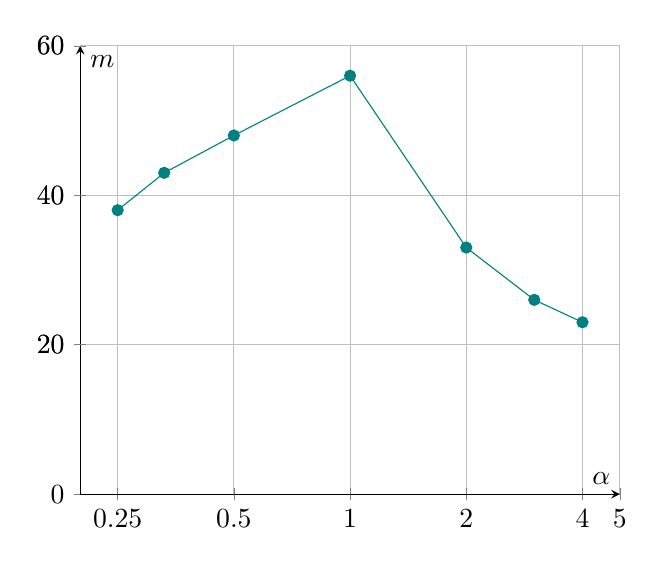
\begin{tikzpicture}
	\begin{semilogxaxis}[
		axis lines=middle,
		axis x line=bottom,  
		axis y line=left,
		xlabel=$\alpha$,
		ylabel=$m$,
		xmin=0.20, xmax=5,
		domain=0.20:5,
		xticklabels={0.25,0.5,1,2,4, 5},
		xtick={0, 0.25,0.5,1,2,4, 5},
		ymin=0, ymax=60,
		extra y ticks ={20,40,60},
		extra y tick labels ={20,40,60},
		grid=major,
	]

	\addplot[mark=*, mark size=2pt, teal, mark color=teal] coordinates {
		(0.25, 38)
		(0.33, 43)
		(0.5, 48)
		(1, 56)
		(2, 33)
		(3, 26)
		(4, 23)
	};

	\end{semilogxaxis}

\end{tikzpicture}

			\caption{Valeur de $m$ en fonction de $\alpha$, avec $q = 1/3$ et
			$\varepsilon = 10^{-6}$}
			\label{fig:result-gamblers}
	\end{figure}
	
	On a décidé de garder $\varepsilon = 10^{-6}$ comme paramètre de sécurité,
	considérant que c'était une bonne valeur de sécurité. Évidemment, plus
	$\varepsilon$ est petit, plus la sécurité est grande, mais la valeur de $m$
	sera plus grande, augmentant ainsi la taille du compressé.

	Bien que l'application des modèles décrit dans les
	articles~\cite{static_backbone} et~\cite{dynamic_backbone} aient prouvés que
	la propriété de qualité de la chaîne n'est respectée que si $q \leq 1/3$ (voir
	la sous-section \ref{subsec:statique-proprietes}), j'ai tout de même prévu de
	faire varier la puissance de calcul de l'adversaire $q \in [0.1, 0.45]$ pour
	voir l'impact de la puissance de calcul de l'adversaire sur la valeur de $m$.
	Prendre en compte cette variation demande encore quelques ajustements dans mon
	programme, c'est pourquoi je n'ai pas encore de résultats impliquant $q \neq
	1/3$ à présenter. La dernière semaine de mon stage sera consacrée à l'étude de
	ces résultats avec un $q \in [0.1, 0.45]$.

	\begin{table}[h]
		\centering
		\begin{tabular}{|c||c|}
			\hline
			$\alpha$ & $m$ \\
			\hline
			$1/4$ & $38$ \\
			% $1/3$ & $43$ \\
			% $1/2$ & $48$ \\
			$1$ & $56$ \\
			% $2$ & $33$ \\
			% $3$ & $26$ \\
			$4$ & $23$ \\
			\hline
		\end{tabular}
		\caption{$m$ en fonction de $\alpha$, avec $q = 1/3$ et $\varepsilon =
		10^{-6}$}
		\label{tab:m_gambler}
	\end{table}


	Le tableau \ref{tab:m_gambler} donne les valeurs de $m$ pour un $\varepsilon =
	10^{-6}$ et un adversaire détenant $1/3$ de la puissance de calcul. La valeur
	de $m$ à choisir sera donc la plus grande des valeurs de $m$ pour chaque
	$\alpha$. La valeur optimale de $m$ sera donc $56$. 
	
	Les résultats sont édifiants : si ils sont validés, ces résultats nous
	permettront d'annoncer qu'il suffit d'attendre $m = 56$ blocs pour être sûr
	que notre bloc ne sera pas invalidé par un adversaire qui triche, peut importe
	la valeur de $\alpha$. Ce résultat est intéressant pour MLS, mais aussi pour
	la chaîne Bitcoin : il est plus rentable pour l'adversaire de "jouer le jeu"
	du protocole et de ne pas faire baisser artificiellement sa target.

	Malgré tout, ces résultats sont à relativiser~: au moment où j'écris ce
	mémoire, nous sommes en train vérifier de manière bien plus formelle que notre
	méthodes et les outils que nous avons utilisés sont bien adaptés au problème
	que nous cherchons à résoudre. Il est donc toujours possible que ces résultats
	soient invalidés par la suite.


\section{Autres travaux}\label{sec:autres-travaux}

	En plus des travaux que j'ai décrit dans les sections précédentes, j'ai
	réalisé quelques travaux satellites qui n'ont pas demandé autant de temps, et
	ne méritaient pas une section à eux seuls.
	
	\paragraph{Communication} Ce stage a été l'occasion pour moi de travailler
	dans le monde de la recherche. J'ai donc eu l'occasion de participer à une
	activité essentielle dans la vie de chercheur : la communication des travaux,
	et le partage des connaissances. J'ai donc eu la chance d'assister aux
	conférences \textit{AlgoTel} et
	\textit{CoRes}\footnote{\url{https://algotelcores2024.sciencesconf.org/}},
	conférences nationales du GDR Réseaux et Systèmes
	Distribués\footnote{\url{https://gdr-rsd.fr/}} sur les algorithmes des
	télécommunications et les protocoles de communication. J'ai pu assister à
	plusieurs présentations, certaines directement liées aux problématiques
	Blockchain. J'ai aussi participé à un séminaire avec toute l'équipe de SOTERN,
	c'était l'occasion de présenter mes travaux, et de discuter des problèmes que
	j'ai rencontrés. J'ai donc fait une présentation de mes travaux, et je me suis
	essayé à l'exercice de la présentation face à un public de chercheurs.
 
	\paragraph{Apprentissage du RUST} Sous les conseils de mon tuteur, j'ai
	commencé à apprendre le langage de programmation RUST quand j'avais le temps.
	J'ai donc appris les bases du langage durant environ une vingtaines d'heures.
	L'apprentissage de ce langage m'aurait permis de travailler sur des
	démonstrateurs de concepts pour MLS ou d'autres protocoles ensuite. Cependant,
	la recherche de $m$ a été bien plus longue que prévu, et ces compétences n'ont
	pas été sollicitées. Malgré tout, c'est un langage de plus en plus utilisé, et
	les concepts et outils qu'il propose sont très intéressants. C'est donc une
	compétence que je suis content d'avoir acquise.
